\scanpage{43}
déformation aux cas du couple $(S_0,S)$, \deleted{\unsure{en}} notant que l'idéal $p\underline O_S$ est bien un idéal à puissances divisées. On notera d'ailleurs que le théorème de déformations dans le cas \deleted{envisagé} général $(S,S')$ envisagé dans son énoncé est en fait équivalent au cas particulier d'un couple $(S_0,S)$, comme il est formel via $\mathrm{Crisloclib}(S)\xrightarrow{\approx}\mathrm{Crisloclib}(S_0)$.

\inserted{\uline{Problème} 3\quad Trouver variante du th. de déformation p\textsuperscript{r} les p-Groupes}
\margin{\figure{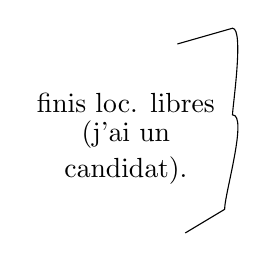
\begin{tikzpicture}
\node[left] at (-.1,0) {\shortstack{finis loc. libres\\(j'ai un\\candidat).}};
\draw (-.7,1.2)--(0,1.4)..controls (.15,1.4) and (0,.4)..(0,.3)..controls (.2,.3) and (-.1,-.7)..(-.1,-.9)--(-.6,-1.2);
\end{tikzpicture}}}

c) F-V-\uline{cristaux admissibles en car.} p. Revenons au cas d'un schéma de car. p. Le cristal de Dieudonné $D^*(G_0)$ étant muni d'une filtration canonique (de $D^*(G_0)_{S_0}$), on pourrait craindre que le problème 1 est mal posé, et qu'il faudrait envisager le foncteur comme étant à valeurs dans des cristaux de Dieudonné filtrés. En fait, dans le cas envisagé ici, il se trouve que la filtration est uniquement déterminée en \unsure{ytermes|termes} de la structure de cristal de Dieudonné, comme on va l'expliquer maintenant.

Considérons le morphisme de topos annelés (qui aura été défini déjà précédemment, dans le par. d'exemples de cristaux, pour les relations entre cristaux et vecteurs de Witt)
\[
\diagram{\begin{tikzcd}
\phi:\quad S_{0\,\unsure{\mathrm{cris}|\mathrm{crys}}/\underline F_p} \arrow[r] & S_0 \arrow[l,bend right=55,"\varepsilon"'] .
\end{tikzcd}}
\]
Soit $M=D^*(G_0)$, et soit $M_0$ sa restriction au site cristallin rel. à $\underline F_p$. Il se trouve que \deleted{la suite} d'après $FV=p$, $VF=p$, les composés dans la suite
\[
\diagram{\begin{tikzcd}
\unsure{M}_0^{(p)} \arrow[r,"F_{M_0}"] & M_0 \arrow[r,"V_{M_0}"] & M_0^{(p)} \arrow[r,"F_{M_0}"] & M_0
\end{tikzcd}}
\]
sont nuls; en fait, on prouvera mieux, à savoir que \inserted{pour tout cristal de Dieud. M,} la suite précédente est exacte (terme à terme sur tout épaississement à p.div. de car.p de $S_0$) et on obtient ainsi des sous-cristaux en modules loc. libres
\[
\operatorname{Ker}V_{M_0}=\operatorname{Im}F_{M_0}\subset M_0,\quad
\operatorname{Ker}F_{M_0}=\operatorname{Im}V_{M_0}\subset M_0^{(p)}.
\]
Ceci dit, \deleted{le sous-Module $\operatorname{Fil}^1$} notons que $M_{S_0}=\varepsilon^*(M_0)$, donc
\[
\phi^*(M_{S_0})\simeq M_0^{(p)}
\]
donc on a
\[
\phi^*(\operatorname{Fil}^1(M_{S_0}))\subset M_0^{(p)}.
\]
Ceci posé, on montre qu'on a
\margin{42}
